% !TEX root = ../main.tex
% Chapter: Results
\chapter{Results}
\label{ch:results}

% Booklet brief: "punchy and dry" -- present results, NO interpretation (that belongs in the
% Discussion). Curate hard: <=20 figures + tables TOTAL across the whole report.
%
% REWIRED 2026-08-14. Ordering principle: the chapter runs PRIMARY -> ABLATION -> CONTEXT,
% not chronologically. The soft-clDice arm and its exact control are the primary result and
% are still training, so they appear as marked placeholders at the TOP, not appended at the
% end. Everything from the from-scratch MONAI era (sealed-test three-model table,
% 128-cubed patches, reduced downsampling, distal sampling, calibre weighting, gap
% reconnection) has been REMOVED to Appendix A.
%
% NAMING: use descriptive arm names in prose (labelled-only seed, MT90, MT240, exposure arm),
% not internal dataset numbers. Internal IDs are kept in comments for traceability only.
% This is a COMPLIANCE point, not a style preference: the Guide states the assessors (at
% least two academic staff besides the module lead) will not have followed the project, so
% unexplained internal shorthand costs marks for clarity.
%
% FIGURE/TABLE BUDGET: 20 combined across the whole body, appendix excluded. Six figures are
% already committed (2 Background/Methods clDice+skeleton, backbone, MT flow, target
% construction, target skeletons). Every FIGURE/TABLE CANDIDATE below must therefore earn
% its slot. The grade rubric rewards figures that "incorporate relevant and ORIGINALLY
% PRESENTED content" -- the paired per-case delta plot and the diagnostics dashboard are the
% two most original artefacts available here, so protect those slots first.
%
% EXCLUDED BY DESIGN -- do not reinstate: the cold-start MT arm whose uniform sampler produced
% warm-up batches with no supervised gradient. That is an implementation fault, not a
% scientific result. It is named once in Methods/Discussion as a protocol lesson and nowhere
% else. Same for the loss-ablation arm that was walltime-truncated at epoch 319/1000 -- if it
% appears at all, it is labelled an early-checkpoint snapshot, never a completed ablation.
%
% ROUGH DRAFT: descriptive only. All "why" statements belong in Chapter 5.
% FORMAT: introduce each display, state only a non-obvious pattern, and never transcribe rows
% of values into prose. The displays carry the numerical record; interpretation belongs in
% Discussion and supporting breakdowns in Appendix A.

% OUTSTANDING RESULTS (2026-08-19). Every item below has a \pending marker in the
% text or a \pending row in a table, so grep for "\pending" to find them all. The
% document must contain none at submission.
%
%   1. Soft-clDice five-fold -- COMPLETE and entered in tab:primary. Its absolute
%      calibre/depth profiles are being regenerated; without a five-fold control it
%      is not used for treatment-minus-control attribution.
%   2. Consistency weight w_max = 0.30 -- COMPLETE and entered in tab:weight-sensitivity.
%   3. Voxel-MSE consistency at w_max=0.30 is scored and entered in tab:primary.
%      Wait for the nominally matched w_max=0.10 arm before adding the objective
%      comparison to a figure. This is the empirical answer to "why a centreline
%      objective rather than a voxelwise one"; its own subsection is retained below.
%   4. Seed snapshots at earlier epochs. HOME: Appendix A, not Results -- it is a
%      probe of when the teacher becomes saturated, not an arm on the primary axis.
%      Exception: if it dates the case-044 break, one sentence in Discussion 4.7.
%   5. 2x upsampled soft skeleton. HOME: row in tab:primary if it is run as a full
%      arm; Appendix A if it stays a cost/gradient probe.
%
% RECOMMENDED FIGURES not yet made, both generatable from data already on disk:
%   A. Calibre delta-TLD (the guide's "Option B"). The calibre section is the only
%      load-bearing analysis with no figure, and the 1-2 voxel band carries the
%      headline. HIGHEST VALUE.
%   B. Paired per-case difference strip, one panel each for TLD, BD, precision,
%      20 points and a mean line. The prose claims the gain is "diffuse rather than
%      carried by a small number of cases" and currently supports that with win
%      counts alone; this is the figure that shows it.

\section{Overall segmentation performance}
\label{sec:primary-matched-pair}

\ifshowcurrentcontrol
\begin{currentcontrolroute}
\noindent\textbf{Current fitted-checkpoint route.}
Primary validation performance is summarised in Table~\ref{tab:primary-current}.

\begin{table}[htbp]
  \centering
  \footnotesize
  \setlength{\tabcolsep}{4.5pt}
  \caption[Current fitted-checkpoint comparison on external validation]{Performance on the
  20-case external validation cohort. Native output is primary; LCC is the connected-component
  sensitivity. Metrics are percentages and differences are percentage points. Differences are
  patient-paired across independently realised checkpoints, not training-seed replicates.}
  \label{tab:primary-current}
  \begin{tabular}{lrrrrcrrrr}
    \toprule
    & \multicolumn{4}{c}{Raw output} & & \multicolumn{4}{c}{Connected component (LCC)} \\
    \cmidrule(lr){2-5} \cmidrule(lr){7-10}
    Arm & Dice & TLD & BD & Prec. & & Dice & TLD & BD & Prec. \\
    \midrule
    16-label seed                  & 92.17 & 91.34 & 83.37 & 92.82 & & 92.62 & 89.51 & 81.38 & 93.99 \\
    110-case-pool scale reference & 92.50 & 93.33 & 88.17 & \textbf{94.91} & & 92.53 & 91.67 & 85.87 & 95.28 \\
    \addlinespace
    Configuration comparator       & 92.64 & 92.02 & 85.47 & 93.57 & & 92.23 & 88.42 & 81.34 & 94.57 \\
    Mean Teacher, fold~0           & 92.25 & \textbf{93.98} & \textbf{89.09} & 94.15 & & 91.56 & 90.43 & 85.09 & 94.91 \\
    Mean Teacher, five folds       & \textbf{92.77} & 93.81 & 88.93 & 94.55 & & \textbf{93.14} & \textbf{92.50} & \textbf{87.21} & \textbf{95.53} \\
    \addlinespace
    Voxel-MSE, $w_{\max}=0.30$     & 92.55 & 91.69 & 84.84 & 93.40 & & 92.29 & 88.23 & 80.96 & 94.66 \\
    \addlinespace
    $\Delta$ MT $-$ control (pp)   & $-$0.39 & $+$1.96 & $+$3.62 & $+$0.57 & & $-$0.66 & $+$2.01 & $+$3.75 & $+$0.34 \\
    \quad cases favouring treatment & 7/20 & 20/20 & 19/20 & 13/20 & & 7/20 & 19/20 & 16/20 & 13/20 \\
    \bottomrule
  \end{tabular}
\end{table}
\end{currentcontrolroute}
\fi

\ifshowpairedcontrol
\begin{pairedcontrolroute}
\noindent\textbf{Prospective paired-seed route.}
\pending[Insert the paired-seed summary table: mean within-seed change, interval and number of
seed pairs favouring Mean Teacher for each metric.]
\end{pairedcontrolroute}
\fi

\section{Airway-tree recovery by calibre}
\label{sec:calibre}

\ifshowcurrentcontrol
\begin{currentcontrolroute}
Figure~\ref{fig:calibre-delta} and Tables~\ref{tab:calibre-td}
and~\ref{tab:calibre-precision} localise the fitted-checkpoint difference by airway calibre. The
TLD difference was concentrated in one-to-two-voxel reference airways; no band at or above five
voxels differed significantly. Prediction-calibre precision fell in the one-to-two-voxel band
and increased in every wider band.

\begin{figure}[htbp]
  \centering
  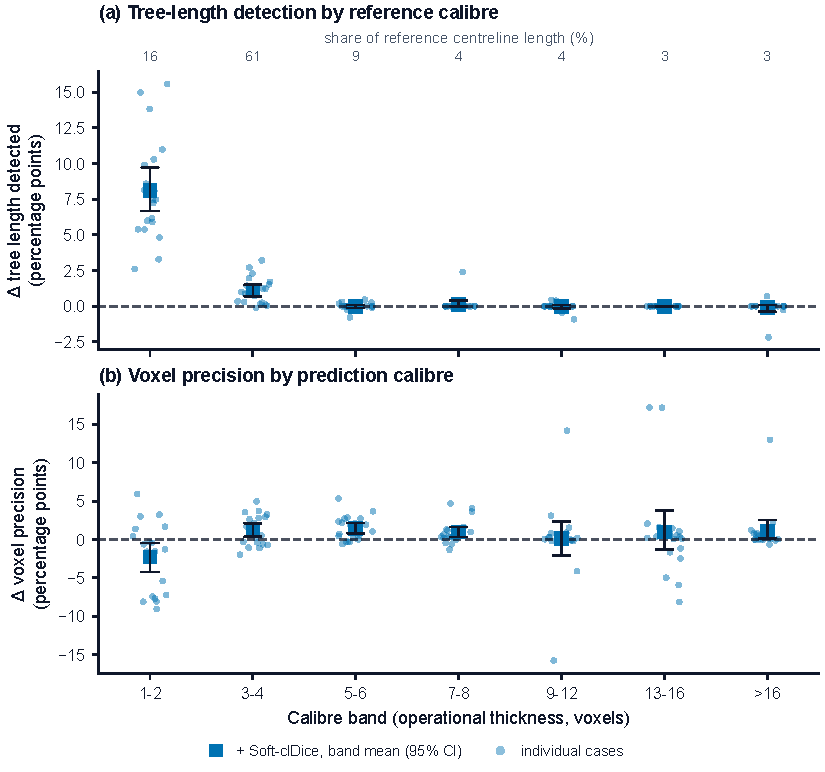
\includegraphics[width=\linewidth]{Figures/pdf/results/calibre_delta_td_noinset.pdf}
  \caption[Tree-length and precision changes by airway calibre]{Paired Soft-clDice minus
  comparator differences on the 20-case validation cohort. A: TLD stratified by reference
  calibre. B: voxel precision stratified by each prediction's own calibre because false-positive
  voxels have no reference calibre. Squares show band means with 95\% patient-bootstrap
  intervals; pale points show cases, and positive values favour Soft-clDice. The upper axis gives
  each band's share of reference centreline length.}
  \label{fig:calibre-delta}
\end{figure}

\begin{table}[htbp]
  \centering
  \footnotesize
  \setlength{\tabcolsep}{2pt}
  \caption[Tree length stratified by ground-truth airway calibre]{Tree length detected by local
  lumen calibre on the external validation cohort. Bands are the exhaustive operational classes
  of Equation~\eqref{eq:opclass}, and ``GT len'' is each band's share of annotated centreline
  length. ``Seed'' is the 16-label initial checkpoint and ``Sup. ref.'' the 110-label scale
  reference. TLD values are percentages and differences are percentage points.}
  \label{tab:calibre-td}
  \begin{tabular}{lrrrrrrrr}
    \toprule
    Thickness & GT len & Seed & Config. & MT & MT & Sup. & $\Delta$ MT & Wins \\
    (voxels) & (\%) & & & fold~0 & 5-fold & ref. & $-$ control & \\
    \midrule
    1--2   & 15.65 & 64.44 & 67.10 & \textbf{75.20} & 73.82 & 70.73 & $+$8.10$^{***}$ & 20/20 \\
    3--4   & 61.34 & 95.23 & 95.68 & 96.77 & \textbf{96.90} & 96.81 & $+$1.09$^{***}$ & 19/20 \\
    5--6   &  9.11 & 99.68 & 99.72 & 99.72 & 99.77 & \textbf{99.78} & 0.00 & 4/20 \\
    7--8   &  3.92 & 99.85 & 99.48 & 99.62 & 99.88 & \textbf{99.93} & $+$0.14 & 2/20 \\
    9--12  &  4.13 & 99.77 & 99.69 & 99.66 & 99.82 & \textbf{99.84} & $-$0.03 & 2/20 \\
    13--16 &  2.56 & 98.47 & 98.50 & 98.50 & 98.53 & \textbf{98.76} & 0.00 & 0/20 \\
    $>$16  &  3.29 & \textbf{96.20} & 96.06 & 95.95 & 94.53 & 93.57 & $-$0.11 & 1/18 \\
    \midrule
    All    & 100.00 & 91.34 & 92.02 & \textbf{93.98} & 93.81 & 93.33 & $+$1.96$^{***}$ & 20/20 \\
    \bottomrule
  \end{tabular}
  \parbox{\linewidth}{\footnotesize $^{***}p<0.001$, Wilcoxon signed-rank; unmarked
  differences $p>0.05$. The $>$16 band uses 18 cases because two contain no voxels in it.}
\end{table}

\begin{table}[htbp]
  \centering
  \footnotesize
  \setlength{\tabcolsep}{3pt}
  \caption[Voxel precision stratified by predicted airway calibre]{Voxel precision stratified by
  each prediction's own local calibre on the external validation cohort. Bands use the
  operational classes of Equation~\eqref{eq:opclass}; prediction-derived classes are required
  because false-positive voxels have no reference calibre. Values are patient-level means in
  percent and differences are percentage points. Arm abbreviations match
  Table~\ref{tab:calibre-td}.}
  \label{tab:calibre-precision}
  \begin{tabular}{lrrrrrrr}
    \toprule
    Thickness & Seed & Config. & MT & MT & Sup. & $\Delta$ MT & Wins \\
    (voxels) & & & fold~0 & 5-fold & ref. & $-$ control & \\
    \midrule
    1--2   & 76.43 & 76.11 & 73.82 & 76.42 & \textbf{78.75} & $-$2.29 &  6/20 \\
    3--4   & 91.56 & 92.42 & 93.69 & 93.91 & \textbf{93.93} & $+$1.27 & 13/20 \\
    5--6   & 94.12 & 94.72 & \textbf{96.19} & 95.74 & 96.05 & $+$1.47 & 15/20 \\
    7--8   & 94.84 & 95.39 & \textbf{96.38} & 96.16 & 96.35 & $+$0.99 & 17/20 \\
    9--12  & 95.87 & 96.28 & 96.42 & \textbf{97.08} & 96.67 & $+$0.14 & 14/20 \\
    13--16 & 95.96 & 95.05 & 96.01 & 95.54 & \textbf{98.43} & $+$0.96 & 14/20 \\
    $>$16  & 92.51 & 95.30 & \textbf{96.37} & 96.30 & 95.79 & $+$1.07 & 15/18 \\
    \bottomrule
  \end{tabular}
  \parbox{\linewidth}{\footnotesize ``Wins'' counts cases with higher precision under fold-0
  Soft-clDice than under the configuration comparator. The $>$16 band uses 18 complete cases;
  overall voxel precision is reported in Table~\ref{tab:primary-current}.}
\end{table}
\end{currentcontrolroute}
\fi

\ifshowpairedcontrol
\begin{pairedcontrolroute}
\noindent\textbf{Prospective paired-seed route.}
\pending[Replace the fitted-checkpoint display with seed-paired calibre differences and
across-seed intervals.]
\end{pairedcontrolroute}
\fi

\section{Airway-tree recovery by branch depth}
\label{sec:depth}

\ifshowcurrentcontrol
\begin{currentcontrolroute}
Figure~\ref{fig:depth-recovery} shows tree-length recovery by reference branch depth. The
fitted-checkpoint difference emerged beyond depth~3 on both validation and held-out cohorts.

\begin{figure}[htbp]
  \centering
  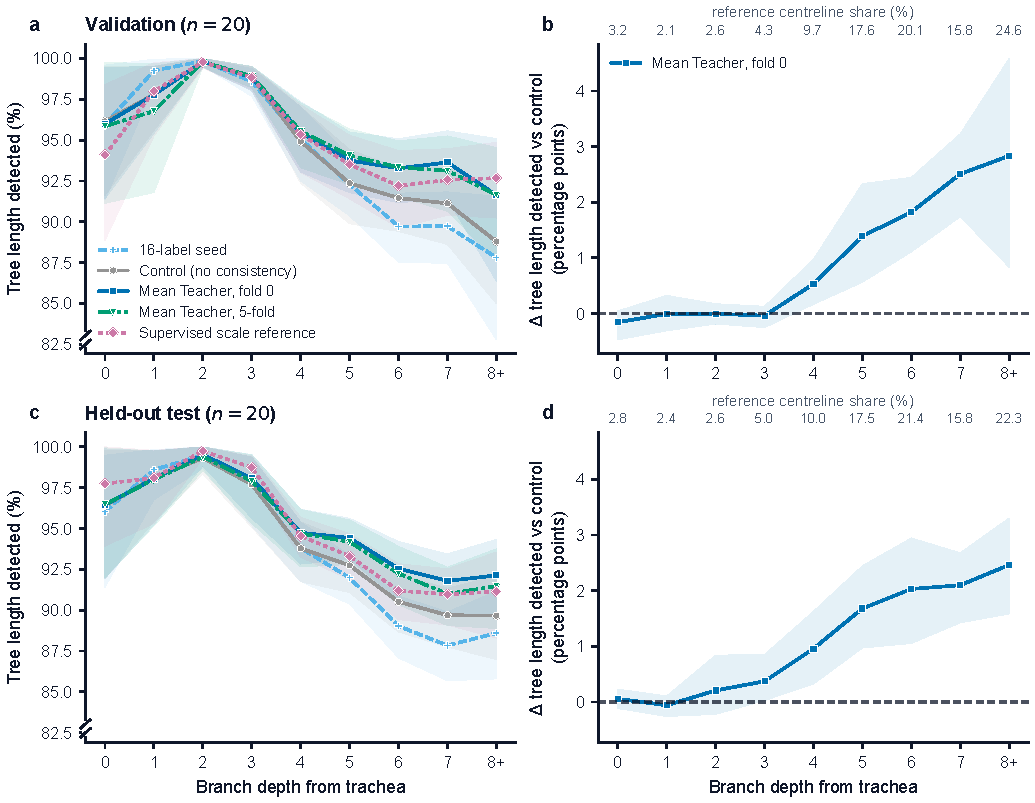
\includegraphics[width=\linewidth]{Figures/pdf/results/generation_depth_recovery.pdf}
  \caption[Tree-length recovery by branch depth]{Branch-depth recovery on the ATM'22 validation (a,b) and held-out test
(c,d) cohorts. Left: absolute tree-length detection percentages, including the 16-label seed
and 110-label scale reference. Right: paired percentage-point difference between the fold-0
Mean Teacher and its configuration-matched no-consistency comparator. Lines and shaded regions
show cohort means and 95\% bootstrap intervals over 20 cases. Depths eight and above are pooled
as $8+$.}
  \label{fig:depth-recovery}
\end{figure}
\end{currentcontrolroute}
\fi

\ifshowpairedcontrol
\begin{pairedcontrolroute}
\noindent\textbf{Prospective paired-seed route.}
\pending[Replace the fitted-checkpoint display with seed-paired depth differences and
across-seed intervals.]
\end{pairedcontrolroute}
\fi

\section{Secondary comparisons}
\label{sec:ablation-mse}
\label{sec:soft-fivefold}
\label{sec:ablation-weight}

\ifshowcurrentcontrol
\begin{currentcontrolroute}
The five-fold ensemble and voxel-MSE arm are included in
Table~\ref{tab:primary-current}.
\end{currentcontrolroute}
\fi
Table~\ref{tab:weight-sensitivity} reports the completed soft-clDice consistency-weight sweep.

\begin{table}[htbp]
  \centering
  \footnotesize
  \caption[Consistency-weight sensitivity]{Fold-0 validation sensitivity to the maximum
  soft-clDice consistency weight. Metrics are percentages. These are single runs;
  $w_{\max}=0.10$ is the reported operating point.}
  \label{tab:weight-sensitivity}
  \begin{tabular}{lrrrrrr}
    \toprule
    $w_{\max}$ & Dice & TLD & BD & Precision & TPrec. & clDice \\
    \midrule
    0.03 & 92.76 & 92.99 & 87.39 & 93.54 & 92.27 & 92.48 \\
    0.10 & 92.25 & 93.98 & 89.09 & 94.15 & 90.57 & 92.08 \\
    0.30 & 92.14 & 95.26 & 91.42 & 93.53 & 86.69 & 90.61 \\
    \bottomrule
  \end{tabular}
\end{table}

\section{External evaluation}
\label{sec:external}

\ifshowcurrentcontrol
\begin{currentcontrolroute}
Held-out ATM'22 and AeroPath performance is summarised in
Table~\ref{tab:external-evaluation}.

\begin{table}[htbp]
  \centering
  \footnotesize
  \setlength{\tabcolsep}{5pt}
  \caption[External evaluation]{Native-output performance on the sealed 20-case ATM'22 test
  cohort and the 27-case AeroPath cohort. Mean Teacher rows use the deployed EMA teacher.
  Metrics are percentages; differences are percentage points comparing fold~0 Mean Teacher
  with the no-consistency comparator.}
  \label{tab:external-evaluation}
  \begin{tabular}{lrrrrr}
    \toprule
    Arm & Dice & TLD & BD & Prec. & clDice \\
    \midrule
    \multicolumn{6}{l}{\itshape Sealed ATM'22 test cohort} \\
    Supervised scale reference & 92.58 & 92.69 & 86.98 & 93.14 & \textbf{92.17} \\
    16-label seed              & 91.84 & 90.63 & 83.14 & 92.11 & 90.86 \\
    No-consistency control     & 92.10 & 91.63 & 85.39 & 92.25 & 91.63 \\
    Mean Teacher, fold~0       & 92.01 & \textbf{93.44} & \textbf{89.18} & 93.30 & 91.47 \\
    Mean Teacher, five folds   & \textbf{92.93} & 93.01 & 88.22 & \textbf{94.19} & 92.00 \\
    $\Delta$ fold-0 MT $-$ control (pp) & $-$0.09 & $+$1.81 & $+$3.79 & $+$1.05 & $-$0.16 \\
    \addlinespace
    \multicolumn{6}{l}{\itshape AeroPath out-of-distribution cohort} \\
    Supervised scale reference & \textbf{84.95} & 94.59 & 92.03 & \textbf{86.28} & \textbf{80.74} \\
    No-consistency control     & 84.22 & 94.46 & 91.20 & 82.56 & 78.50 \\
    Mean Teacher, fold~0       & 84.24 & 95.03 & 92.52 & 83.99 & 76.18 \\
    Mean Teacher, five folds   & 84.90 & \textbf{95.41} & \textbf{92.73} & 84.67 & 77.76 \\
    \addlinespace
    $\Delta$ fold-0 MT $-$ control (pp) & $+$0.02 & $+$0.57 & $+$1.32 & $+$1.43 & $-$2.32 \\
    \bottomrule
  \end{tabular}
\end{table}
\end{currentcontrolroute}
\fi

\ifshowpairedcontrol
\begin{pairedcontrolroute}
\noindent\textbf{Prospective paired-seed route.}
\pending[Insert seed-paired external-evaluation table for held-out ATM'22 and AeroPath.]
\end{pairedcontrolroute}
\fi
